%%%%%%%%%%%%%%%%%%%%%%% file template.tex %%%%%%%%%%%%%%%%%%%%%%%%%
% $Id: woc_2col.tex 158 2017-01-19 23:08:23Z foley $
% $URL: https://repository.cs.ru.is/svn/template/tvd/journal/matec-woc/woc_2col.tex $
% 
% This is a template file for Web of Conferences Journal
%
% Copy it to a new file with a new name and use it as the basis
% for your article
%
% This template has been updated to match the Word Template's contents
% by Joseph T. Foley < foley AT RU dot IS >
%
%%%%%%%%%%%%%%%%%%%%%%%%%% EDP Science %%%%%%%%%%%%%%%%%%%%%%%%%%%%
%
%%%\documentclass[option]{webofc}
%%% "twocolumn" for typesetting an article in two columns format (default one column)
%
\documentclass[twocolumn]{webofc}
\usepackage[varg]{txfonts}   % Web of Conferences font
\usepackage{booktabs}
\usepackage{algorithm}
\usepackage{float} 
\usepackage{listings}
\usepackage{algpseudocode}
\usepackage{array} %% needed for advanced table manipulation
%% Column types from http://tex.stackexchange.com/questions/54069/table-with-text-wrapping
\newcolumntype{L}[1]{>{\raggedright\let\newline\\\arraybackslash\hspace{0pt}}m{#1}}
\newcolumntype{C}[1]{>{\centering\let\newline\\\arraybackslash\hspace{0pt}}m{#1}}
\newcolumntype{R}[1]{>{\raggedleft\let\newline\\\arraybackslash\hspace{0pt}}m{#1}}

\graphicspath{{graphics/}{graphics/arch/}{Graphics/}{./}} % Look in these folders for graphics
%
% Put here some packages required or/and some personnal commands
%
%
\begin{document}
%
\title{Final report of 540 Machine Learning}
%
% subtitle is optionnal
%
%%%\subtitle{Do you have a subtitle?\\ If so, write it here}

\author{\firstname{Guangyuan} \lastname{Yu}\inst{1}\fnsep\thanks{\email{gy12@rice.edu}} \and
        \firstname{Andrew} \lastname{Wells}\inst{2}
        % etc.
      }

\institute{Physics and Astronomy, Rice University, Houston, 77006, Tx, USA
\and
           computer science, Rice University, Houston, 77006, Tx, USA
          }

\abstract{%
We build a 11 layer CNN and achieved 97.8\%accuracy on the SVHN public data set and 98\%1 for private set, standing 5th. We use local response normalization and shortcut to improve the performance of backward parameter tuning process. 
In this report, we will show our machine learning
framework, preprocessing procedures and experiments on several
models, including Convolutional Neural Network, Residual Neural Network and our model. Furthermore, a deeply discussion is given at the end of this work.
Keywords?Picture Preprocessing, Machine Learning Models, CNN, Alexnet, ResNet, model Ensemble.
  
}
%
\maketitle
%
\section*{Introduction}\label{sec:readme}
\textbf{SVHN is a real-world image dataset for developing machine learning and object recognition algorithms with minimal requirements on data pre-processing and formatting. SVHN is obtained from house numbers in Google Street View images. This dataset includes three parts: A training set with 73,257 digits, an extra data set with 531,131 digits and 26,032 digits for testing. Fig 1 shows some data sample, all the data are in 32*32 RGB format. The training and extra data set are labeled from 1 to 10, which indicates the number in the center of the picture, where a label of 10 means the digit is a '0'. \\
We get an 97.89\%  accuracy by using a convolutional neural network (CNN). CNN's(FIG 2) are variations of multilayer perceptrons designed to use minimal amounts of preprocessing. CNN's  have wide applications in image and video recognition, recommender systems, and natural language processing.
}




\begin{figure}[H]
  \centering
  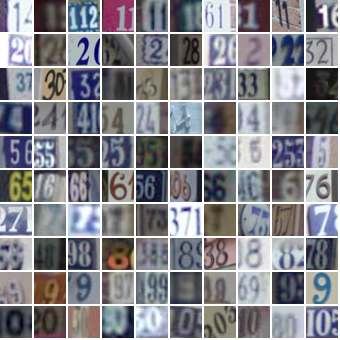
\includegraphics[width=0.6\columnwidth]{3232.png}
  \caption{SVHN dataset.}
\end{figure}


\begin{figure}[H]
  \centering
  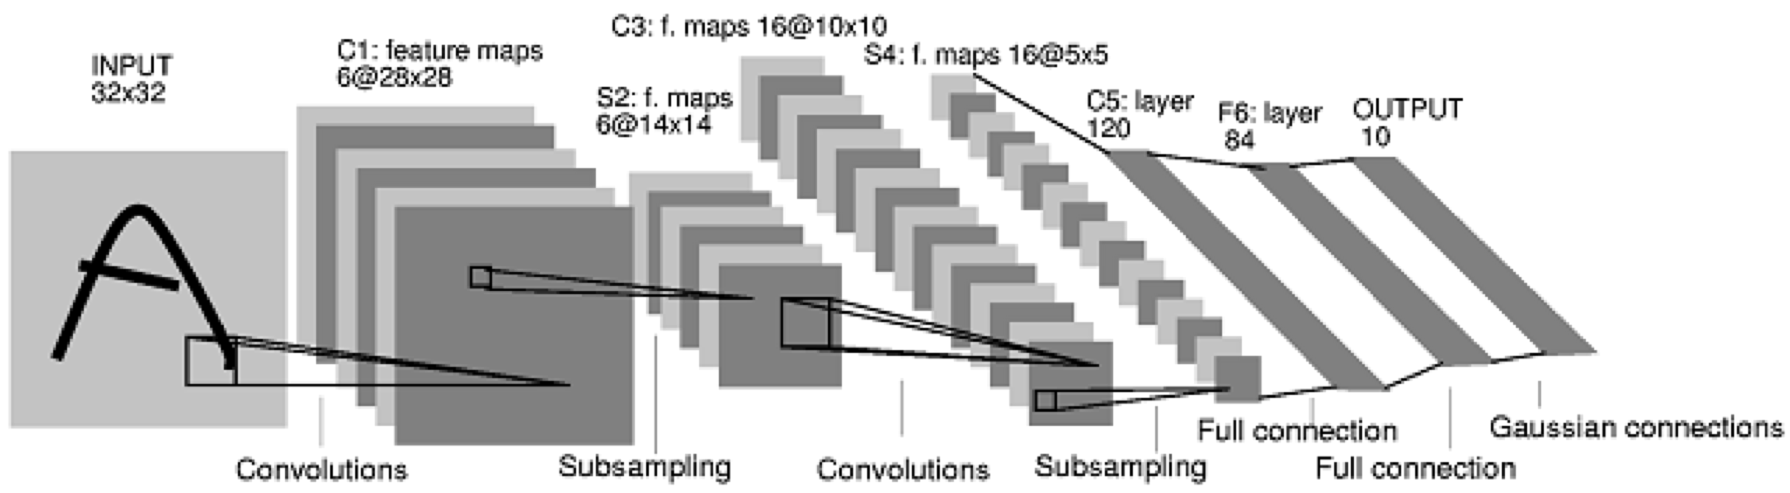
\includegraphics[width=\columnwidth]{cnn.png}
  \caption{CNN structure.}
\end{figure}

\section{Our model}
\subsection{Final approach}
The structure is in Fig4. It is a 10 layer CNN followed by 2 layer FC. The channel number is 32-32-32-48-64-128-128-128-256-256-2048-10. The filter size is 5,5,5,3,3,3,3,3,3,3.
We use ReLU, local response normalization,voter(ensemble), our final standing is 5th for private set, 6th for public set(except the wrong 1st place). Final public accuracy is 97.8\%, private 98.1\%.



\subsection{data pre-processing}
The color information is not important here. So we change the picture into gray scale. Fig 3 shows the gray scale.
\begin{lstlisting}
data=R*0.3+G*0.59+B*0.11
data=data-mean of a single picture
data=data/std of a single picture

\end{lstlisting}

\begin{figure}[H]
  \centering
  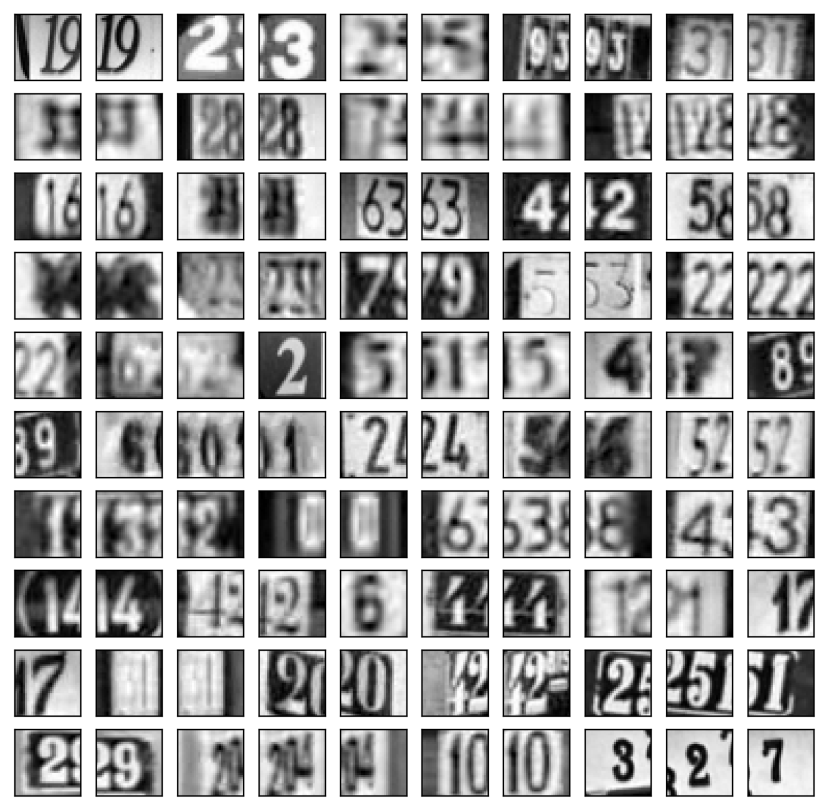
\includegraphics[width=0.6\columnwidth]{gray.png}
  \caption{data pre-processing}
\end{figure}



\subsection{How to select the feature:?}\label{sec:formatting}
After searching the Internet, we find that deep learning approaches, usually the Convolutional Neural Network\cite{Krizhevsky2012b,Ciresan2011} or similar network have very good performance. Good examples, include Alexnet and ResNet. I tried both, and though I expect the ResNet\cite{Szegedy} should have better performance, but my computer could not build a 150-layer net so I tried from 10 layers to 50 layers and get an accuracy of 95.5\% Due to the limited time I can't make it better because I already spent a lot of time on AlexNet. 
At the beginning I use a 2 layer CNN as the Tutorials in TensorFlow said. It is easy to get good performance on MNIST database because the background of handwritten letters are all black and the size of the letter are similar to each other. However, our SVHN dataset are complicated; some letters are big, some of them are small and there's a lot of irrelevant stuff in the picture. So the 2 layer CNN could not get a good performance on the SVHN. So I change it to a six layer network. For practical purposes, we want to use $2^n$ number of channels. Typically increasing the channel numbers gradually will have a better result, so I stared from 32 channels and stop at 512 channels. 
With a 6 layer CNN, we can get about 94\% accuracy on training set and 96\% accuracy with extra dataset. 
The six layers I use are 64-128-128-128-128-256, followed by a fully connected layer 4*4*256-256-10 softmax.
To improve it, the net can be made more complicated even though it is harder to train. 
Deeper networks have some issues. We cannot guarantee deep net will preform better than the shallow net because the training process, especially the gradient transfer process is difficult. That is why ResNet was invented. It solves this problem by adding shortcuts in the net. So ResNet look like a net containing many small nets. To improve my net, I use this short cut feature and combine it with my "AlexNet". It is a 11-layer CNN with shortcuts and a fully-connect layer. I also tried 15 layers but it is worse than 11 layers. 
The 11 layer is 32-32-32-64-64-64-128-128-128-256-256-2048-10. For the filter, the first 3  layers use 5*5 filter, other layers use 3*3 filter. Small filter can get better feature of the curve or edge at the picture but small filter also has smaller view through previous layers. For example, a 3*3 filter at the second layer can see 3*3 pixels in previous layer and 5*5 pixels in two layer before. While a 5*5 filter can see 7*7 pixels in two layer before. So the first few layer should be large filters.
Padding is also important. Without padding, in the middle layers the information at the edge will be collected less time than the information in the center, since it is a deep network, this effect adds up and passes back to the pixels at the original center, which means we don't fully use the information we collected. So we need padding. As another advantage, padding keeps the dimension the same as before. 

After the poster, I get inspired by other group and tried the 10 layer network which has fewer channels. And the result is better than my previous result. I think the problem of my previous net is that the channel This net is 32-32-32-48-48-64-64-128-128-256-256-2048-10, which is my final approach as shown in Fig 4.




\begin{figure}[H]
  \centering
  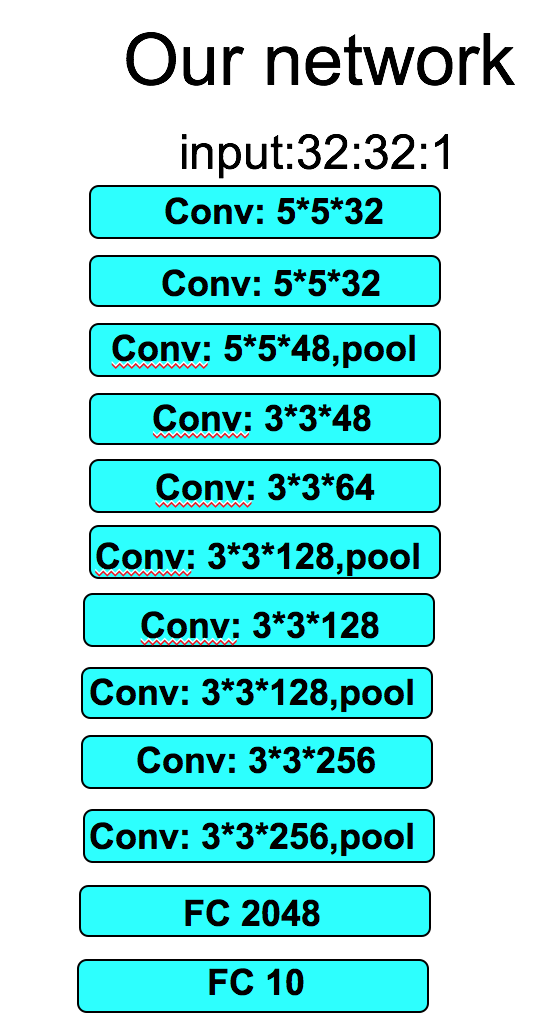
\includegraphics[width=0.6\columnwidth]{ourmodel.png}
  \caption{Our model with best perforamance.}
\end{figure}







I tried all the combinations of leaky ReLU, ReLU and local response normalization, and ReLU with local response normalization had the best performance. I also tried max and fractional pool. With fixed training epoch, max pool usually has better performance but fractional pool can lead to a lower loss function with larger training epoch so I finally choose the fractional pool. There is a dimension difference between max pool and fractional pool: Max pool works in fixed 2d plane and repeats working in the third dimension. So you can feed the function with different batch size, because max pool don't care about the third dimension but for fractional pool the third dimension will be fixed, you can not change the batch size. 

\subsection{Training result}
We get an accuracy of 97.8\% accuracy. 
Fig.5 shows the trained weight of the first layer. We put a sample(Fig 6) into the net and see how the channel get the feature. 

\begin{figure}[H]
  \centering
  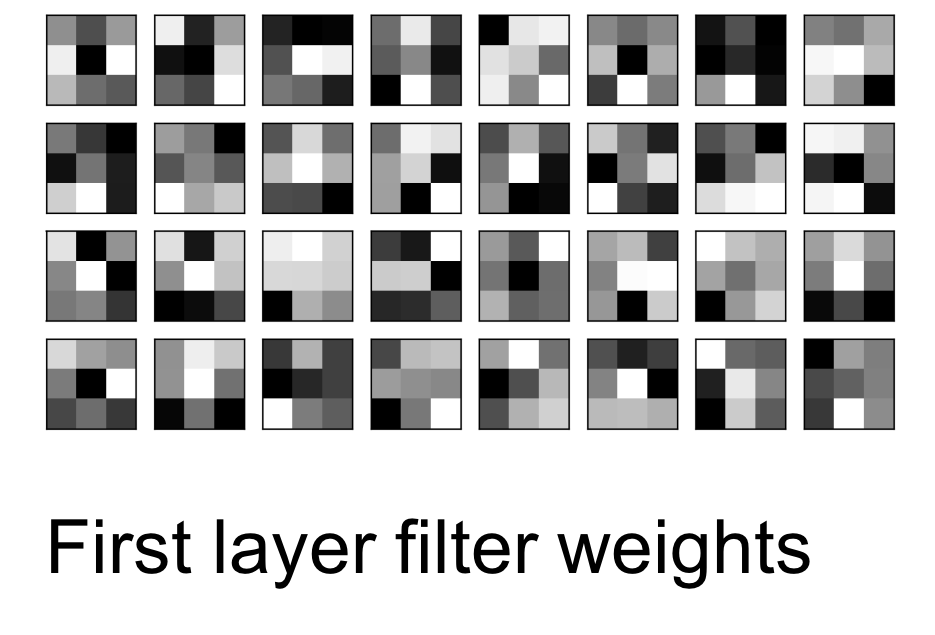
\includegraphics[width=\columnwidth]{weitpng.png}
  \caption{Weight of the first layer}
\end{figure}
\begin{figure}[H]
  \centering
  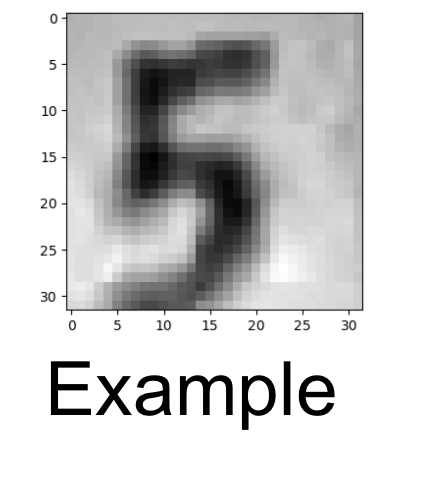
\includegraphics[width=0.6\columnwidth]{sample.png}
  \caption{sample picture}
\end{figure}
As shown in Fig 7, the 32 channels get different features of the input. These channels are slightly different from each other which means they emphasize different features of the input. 

\begin{figure}[H]
  \centering
  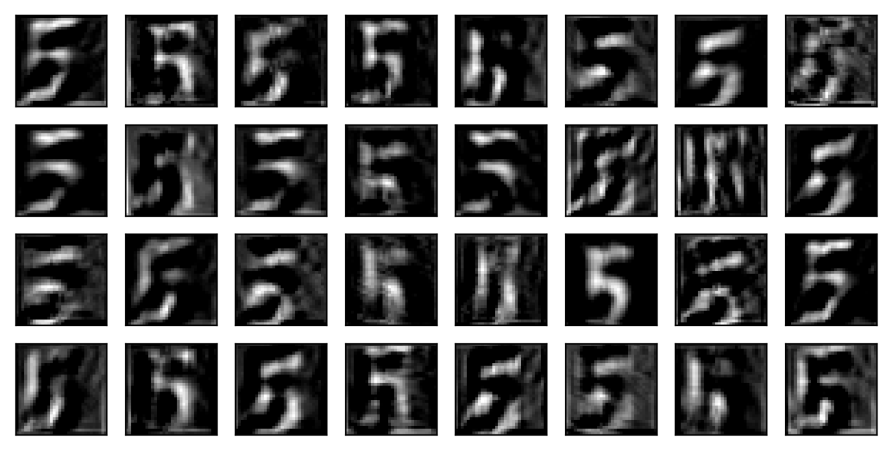
\includegraphics[width=\columnwidth]{Picturefitlter.png}
  \caption{Filter of the first layer}
\end{figure}


\begin{figure}[H]
  \centering
  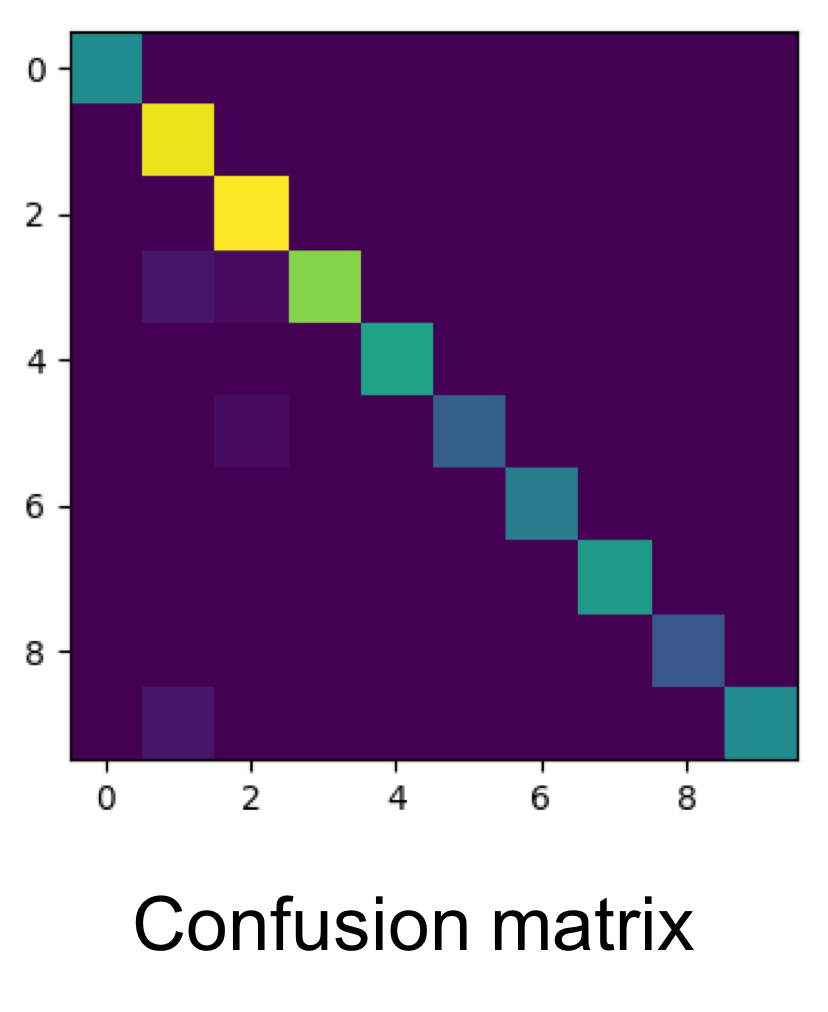
\includegraphics[width=0.6\columnwidth]{softmax.png}
  \caption{The confusion matrix}
\end{figure}
The confusion matrix shows the the prediction is very precise as the pixels on the diagonal are highlighted.


\subsection{A discussion about model assessment:
}\label{sec:formatting}
For over fitting it usually happens at the fully connected layer. Clearly this layer contains more parameters compared to the other single layer. By using the "dropout\cite{Srivastava2014}" parameter in tensorflow we can solve the problem of over fitting. Dropout parameter can be 1, meaning all the parameters will be used.  So in the training process, I change the dropout and when making predictions, the parameter will be set to 1. In the training process, I tried different dropout parameter, finding out 0.5 is too large for the system, leading to may parameters not being trained very well, while 0.7 is a better number, which means 0.7 parameters will be kept in the training. 
Another approach to prevent over fitting is to simply look at the screen. Once I find over fitting occurs, I will stop the training and changing the learning rate. 
To changing the learning rate I tried to write it as a piecewise function. Like first 3 epoch on training set is with lr=1.5e-4 is enough to get accuracy of 90\%, we need to lower it to prevent over fitting so lr=1e-4 for extra data first epoch and 0.8e-4 for 3 extra data epoch. But when I am changing the model, the boundary also needed to be changed, so I finally give up this method in the competition. 
\subsection{A discussion of model selection.
}\label{sec:formatting}

 
At the very beginning I used some method to process the data. Changing it into grayscale, covering the 7 column pixels on the left and right sides, flipping the picture if the background is brighter than the number, using a threshold to distinguish the background, this results in binarization. I also shift the image 1 or 2 pixels up, down, left and right to generate more data. This is because a camera could have been pointed slightly differently and gotten such a picture. The overall impact is very small. I didn't use PCA or whitening, because some website says CNN doesn't need this. Flipping and covering the edges may help 1 to 2\% percent when the accuracy is relatively low, but when the accuracy if over 95\%, they can be neglected. This is partially due to the fact that I can't flip all the data correctly.
Then the table.
The binarization of picture may be used in character segmentation, but since our data set is not clear enough, binarization will make the performance worse. 
Covering doesn't help in the deep network. This is the advantage of deep learning, by using large amount of training data, the network can ignore the influence of irrelevant pixel regions.

As for the model, deeper net have better performance and the net with smoothly increasing channel number is better. 




\subsection{How do I select the approach for the final submission
}\label{sec:formatting}

For this competition, the public depends on 80\% of submitted data. It really shows how accurate the prediction is, because it is 80\%. If it is 1\%, I would not believe the public performance. My validation set is a slice from training set, usually when the validation accuracy is 1\% lower than my submission score. I think it is because the test set is easier than the training set. During this project, I notice that the extradata set is easier than the training set. That is why the training accuracy on extradata usually is 1-2\% higher than the train set. So I just see my validation accuracy, when it is really high, I use the voter to make a prediction and repeat to use the voter many times, then we select the best 4 public performances. 
For the final submission, I just select the top 4 performances from the submission history.



\subsection{What lessons did you learn about solving prediction problems using ML and large data set?}\label{sec:formatting}
1. GPU is so important. My final model needs my GPU to train for about 1 day. The top entries all use good GPU. One of the GPU is even a commercial version.\\
2. Net structure is more important than parameters. There is a limit of accuracy for a specific net, but you don't know the limitation until you reach it. Choosing the net is similar to choosing a dead-end road, you won't realize it until you can't go forward. \\
3. The best parameter and structure is just for a specific data set. When the dataset is changed, both the structure and parameters need to be changed. \\
4. Larger data sets help a lot. But, changing the position of 1 or 2 pixel won't help. My 11 layer can recognize a number 8 far from the center, while my 6 layer can't. Actually this number 8 really bother me a lot, but the benefit of generating artificial data can be covered by make the net deeper. Large original data helps a lot. The 6 layer net without extradata can get 93-94\%, 6 layer net with extra data can get 96\%. \\
5. Writing the data in binary code. I find that when doing homework, we load the cifar10 data set in 1 second, but when loading our SVHN training numpy array data, it takes several minutes not to mention the large extra data. So I also write the training data it to binary code. Note that python2 and python3 use different binary encodings. I cut the extra set into 11 piece and the first 10 piece each have 50000 data. The last have very few data so I never use it.\\
6. Machine learning is a good substitution of the picture processing, even though we still need to handle the picture to feed the machine, but the work is much smaller than before. \\
7. CNN goes deeper and deeper rather than boarder. With more filters, the machine can get the feature of a specific region more precisely, so the width and height of the layer can be smaller and smaller. \\
8 The fully-connect layer is very important for CNN. This layer contains most parameters in the network. Compared with my 20 layer Res model which is deeper but don?t have the FC layer, the FC layer is much more useful. Some paper also mention that the Res works better when it is extreme deep, I think this is the reason my Res doesn?t works well. The number of node should change gradually, for example, the input of FC is 49*256. The hidden layer is 2048 and the output is 10. If there is not hidden layer, the result would be very bad.  And 512 unit is not enough.\\ 
9. Shuffling the data and making random choices from the data doesn?t help anything for our network. I don?t know why there are so many people saying shuffling will help. \\
10. My machine has more prediction accuracy than me. For example, in Fig 9, the wrong prediction actually is really hard to recognize.\\
\begin{figure}[H]
  \centering
  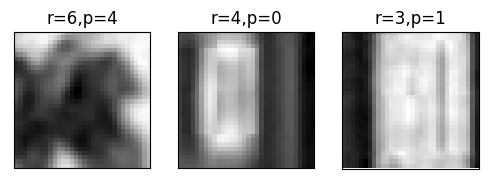
\includegraphics[width=0.6\columnwidth]{wrong.png}
  \caption{The wrong prediction.}
\end{figure}
11. There is no guideline for fine tuning the net. Like the leaky Relu, some people say it helps, some say no. How do you find the best parameters? It is a matter of luck. Trying for a longer time is the only way to reliably get better parameters. \\
12. The adam solver is better than SGD. \\
13. In class, we learned that voters works well in machine learning, and I find a way to use it in CNN. \\
14. When to use the pooling function? We have 11 layers, and want to pool 3 times, we should put the pooling function\cite{Zeiler2013} every three layer. I won?t recommend to pool after the first layer because it will lose a lot of information. And I won?t recommend to put 2 pooling layers together, because it will lose a lot of information. I don?t think pooling to much time to make the output of CNN to 1*1*channels is a good idea. My experiment indicate it is worse than 4*4*channels. I still need to figure out why 1*1 is used in ResNet. \\
15. One possible approach is to use PCA to strength the week data. We know there are many unclear pictures in the train set. I read a Chinese paper where they mention they use PCA by grouping all number 1 together so that some unclear number 1 will be strengthened. \\
16. The result also depends on how good the training set is. The MINST data set can easily get over 99 percents. I used the rotation of the data of 5 degree both to the left and right. But I don?t see the improvement. I think it is because some oblique pictures will become worse. \\
17. I think shuffling or making random choices for the training set didn?t help anything.\\
18. I think the prediction process is not determinative. We save the model. When we load the parameters and make predictions, the prediction can be different from time to time. For example, from 98\% to 95\%. It is a huge difference. This stochastic process does not come from the fractional pool because max fractional poor or average fractional pool are all decisive. I attribute this stochastic variation to the large number of parameters, I mean the calculation noise. The pooling function just magnifies the fluctuation but it is not the source of fluctuation. \\
19. It is a competition, luck is important. The accuracy of teams are very close to each other. The fluctuation of the same bunch of parameter can lead to maybe 0.2\% difference. Small learning rate and dropout can?t grantee that more training will bring better results. It is very important that you make the prediction at a lucky moment when your parameters are at a good value. \\
20. At the last day, the ResNet makes better performance on the kaggle leader board.I have been waiting for this moment for a very long time. The ResNet substitutes the FC layer with a longer network. Which one is better? It depends on how deep is the ResNet. \\
21. I see on the Internet saying that the pre-processing should use the data minus the mean of the whole dataset, I think it is very irresponsible to say that. I see another group using this technique and the result is bad. \\
22. During the poster, I see other groups use some technique that train the opposite pictures during the training process. And both predict the original and opposite test set. It is a good idea. 
23. Other groups add drop out between the layers of ResNet, which helps to solve the over fitting.
24. The fully connected layer actually is also a kind of CNN, the size of filter is 1*1. \\
\begin{figure}[H]
  \centering
  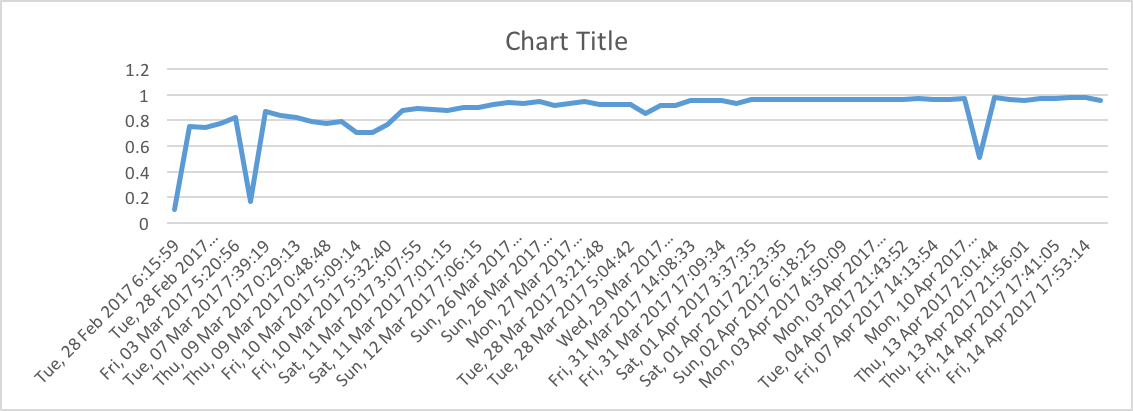
\includegraphics[width=\columnwidth]{performance.png}
  \caption{Team performance history}
\end{figure}



\subsection{What can I do to improve my performance if I had longer time}
1. I would like to crop the pictures which will give the data set more variation and prevent over-fitting. 
2. I will build a deep ResNet with fewer channels at the beginning, I mean 16 channels instead of 32, because our input is small, compared to 267*267. 
3. I will use L2 normalization.  

\section{Performace history}
\begin{table}
  \centering
  \caption{Font styles for a reference to a journal article.}
  \label{tab:font-styles-reference-journal}
  \begin{tabular}{C{25mm}p{25mm}}\toprule
    \textbf{structure} &\textbf{performace}\\\midrule
    10 CNN+FC +lrn+extra +VOTER+fraction pool &97.89\\
    11 CNN+FC +Res+lrn+extra +VOTER+fraction pool &97.7\\
    6 CNN+FC+ extra +lrn+fraction+voter & 96.6\\
    6 CNN+FC+ extra+leaky Relu+fraction & Around 96\\
    6 CNN+FC+ extra+maxpool &96.2\\
    50 LAYER  Res+extra &95.5\\
    20 Layer Res+extra &92.3\\
    20 Layer Res+FC &Not good. \\
    6CNN+FC+FLIP&94.5  \\
    6CNN+FC+COVER&93.8  \\
    6CNN+FC&94.2  \\
    2 CNN+FC+COVER&89.9  \\
    2 CNN +FC&88.7  \\
    2 CNN+ binaryzation&76.9  \\
    2 CNN WITHOUT PADDING &78  \\
    
    \bottomrule
  \end{tabular}
\end{table}







A discussion about why they perform like the way in the table. 
First I want to compare the Res and Alexnet. My 50 or 20 Layer Res net has a problem of over fitting. The training accuracy can get to 1 in the third training epoch which is much faster than Alexnet, but the validation accuracy is around 90, by changing the learning rate, I can improve the accuracy to 95.5, but can?t increase it anymore. I don?t know how to make it better, but I know the poor performance comes from over-fitting. 
Second, in the Alexnet, we can see a clear trend that deeper networks are better than shallow networks. 
Let's start form the bottom, the padding helps to keep the shape and won?t lose the information of center in the backpass process. Without padding, bad performance will occur. 
Binarization: it will make the number more hard to recognize because the the threshold is so hard to choose. But the slope of the learning is much larger than others. It is easy to train.
Flip helps a little because it will make the pictures more consistent. 
Cover helps little because the CNN is powerful enough to overcome the irrelevant staff.
6 layer CNN is much better than 2 layer CNN with improvement of 4-5 percent. The next big improvement occurs when using the extra data.
Large data works! It will bring a 2\% improvement compared with a pure 6 CNN. 
The voter combined with fraction pool brings a little improvement because taking averages will reduce the variance of prediction. 
Compared with 6-layer CNNs, 11-layer CNNs works better but the improvement is not very much. We tried a structure with 10 layers in the last day, which has 48 channels, and the performance is slightly better. 







The training process will take about 1 day. We eventually use a voter to generate a better result. The net can get a stable accuracy of more that 97\% and the voter can improve it by 0.4\%. These two number are my estimation because I always use the voter. The way I run my code is like this: I look at my screen to check the validation accuracy. When the validation is high, I store the model and make a prediction, I store the weight of different of number possibilities into the parameter called "pred", and continue to run the model; when it is above 96.5, I write the possibility into "pred". After repeating several times, I then get the number that has the largest possibility.









\section*{Online URL reference }



\begin{lstlisting}
https://www.tensorflow.org/tutorials/deep_cnn
https://arxiv.org/pdf/1512.03385.pdf
http://cs231n.github.io/convolutional-networks/
https://en.wikipedia.org/wiki/Convolutional_neural_network
\end{lstlisting}




% of note, the template example has a nonexistant reference #3
% Deluca didn't produce a book on his own only as an editor as part of a series
% --foley

%
% BibTeX or Biber users please use (the style is already called in the class, ensure that the "woc.bst" style is in your local directory)
% \bibliography{name or your bibliography database}

\bibliography{fp}





\end{document}

% end of file template.tex
%%%%%%%%%%%%%%%%%%%% TeXStudio Magic Comments %%%%%%%%%%%%%%%%%%%%%
%% These comments that start with "!TeX" modify the way TeXStudio works
%% For details see http://texstudio.sourceforge.net/manual/current/usermanual_en.html   Section 4.10
%%
%% What encoding is the file in?
% !TeX encoding = UTF-8
%% What language should it be spellchecked?
% !TeX spellcheck = en_US
%% What program should I compile this document with?
% !TeX program = pdflatex
%% Which program should be used for generating the bibliography?
% !TeX TXS-program:bibliography = txs:///bibtex
%% This also sets the bibliography program for TeXShop and TeXWorks
% !BIB program = bibtex

%%% Local Variables:
%%% mode: latex
%%% TeX-master: t
%%% End:
